\subsection*{Model}
The function described in this problem is the following
\begin{equation*}
    \begin{aligned}
    & F(\mathbf{x}) = \frac{1}{2} \sum_{k=1}^{n} f_k^2(x) \\
    & f_k(\mathbf{x}) = 10 \left(x_k^2 - x_{k+1}\right), \quad  & \mod (k,2) = 1\\   
    & f_n(\mathbf{x}) = x_{k_1} -1, \quad & \mod(k,2) = 0
    \end{aligned}
\end{equation*}
where $n$ denotes the dimensionality of the input vector $\mathbf{x}$. As convention, we set $x_{n+1} = x_1$ when it is necessary, that is when the dimensionality $n$ is an odd number.
\\ The starting point for the minimization is the vector $\mathbf{x}_0 = [-1.2, 1, -1.2, 1, \ldots]$.

In order to compute the derivatives of this problem we have to consider separately the cases when $n$ is even or odd. In the first case, the gradient of the function is given by
\begin{align*}
    &\frac{\partial F}{\partial x_k} (\mathbf{x}) = \frac{\partial}{\partial x_k} \left[\frac{1}{2} f_{k-1}^2(\mathbf{x})\right] = - 100 (x_{k-1}^2 - x_k) \quad & \mod(k,2) = 0 \\
    & \frac{\partial F}{\partial x_k} (\mathbf{x}) = \frac{\partial}{\partial x_k} \left[\frac{1}{2} f_{k}^2(\mathbf{x}) + \frac{1}{2} f_{k+1}^2(\mathbf{x})\right] = 200x_k (x_k^2 - x_{k+1}) + (x_k -1)\quad & \mod(k,2) = 1
\end{align*}

If the dimensionality $n$ is odd, the only changement is in the first component of the gradient, which becomes
$$ \frac{\partial F}{\partial x_1} (\mathbf{x})  = \frac{\partial}{\partial x_k} \left[\frac{1}{2} f_{k}^2(\mathbf{x}) + \frac{1}{2} f_{k+1}^2(\mathbf{x}) + \frac{1}{2}f_n^2(\mathbf{x}) \right] = 200x_1 (x_1^2 - x_{2}) + (x_1 -1)  - 100(x_n^2 - x_1)$$

Looking at the structure of the problem we are considering, it is obvious that the Hessian matrix is a sparse matrix whose particular structure depends again on wheter $n$ is even or odd. In the first case, the Hessian is a block tridiagonal matrix with the following non-zero terms
\begin{align*}
    \frac{\partial^2 F}{\partial x_k^2} (\mathbf{x}) &= 100, & \frac{\partial^2 F}{\partial x_k \partial x_{k+1}} (\mathbf{x}) &= 0, & \frac{\partial^2 F}{\partial x_k \partial x_{k-1}} (\mathbf{x}) &= -200x_{k-1} & \mod(k,2) &= 0 \\
    \frac{\partial^2 F}{\partial x_k^2} (\mathbf{x}) &= 600x_k^2 - 200x_{k+1} + 1, & \frac{\partial^2 F}{\partial x_k \partial x_{k+1}} (\mathbf{x}) &= -200x_k, & \frac{\partial^2 F}{\partial x_k \partial x_{k-1}} (\mathbf{x}) &= 0 & \mod(k,2) &= 1 \\
\end{align*}

If $n$ is odd, there are two changements in the Hessian matrix: the derivative $\frac{\partial^2 F}{\partial x_1^2} (\mathbf{x}) $ is affected by the presence of $x_1$ in the term $f_n()$ and the extremal diagonals are not zero anymore. We report the terms of the Hessian matrix that differs from the previous case
\begin{align*}
    \frac{\partial^2 F}{\partial x_1^2}  (\mathbf{x}) &= 600x_k^2 - 200x_{k+1} + 101 \\
    \frac{\partial^2 F}{\partial x_n \partial x_1} (\mathbf{x}) &= \frac{\partial^2 F}{\partial x_1 \partial x_n} (\mathbf{x}) = -200x_n
\end{align*}


By analyzing the derivatives of the problem, we can deduce that the gradient of the function is nullified by the vector composed of ones which also nullifies the value of $F(\mathbf{x})$. 


 
\medskip
\subsection*{Nealder Mead Method}
\begin{figure*}[htbp]
    \centering
    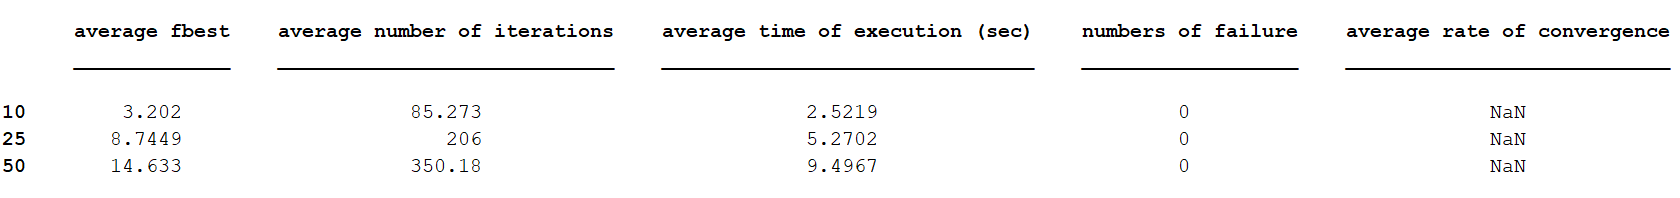
\includegraphics[width = 0.9\textwidth]{img/pb25_SX_table.png}
    \caption{Results obtained by running the symplex method on the problem $25$.}
\end{figure*}
We now report a table showing some general results obtained by running the Nealder Mead method on the problem.

Looking at the table, it is clear that even if the method satisfies the stopping criterion for all dimensionalities does not converge to the minimum point, actually the minimum value it finds increases with the dimensionality.
We are not too surprised by the por performance of the symplex method because the algorithm solely relies on function evaluation and does not take advantage of the information contained in the derivatives of the objecive function.


\medskip
\subsection*{Modified Newton Method - Exact Derivatives}
We now report a table showing some general results obtained by running the Modified Newton method on the problem.
\begin{figure*}[htbp]
    \centering
    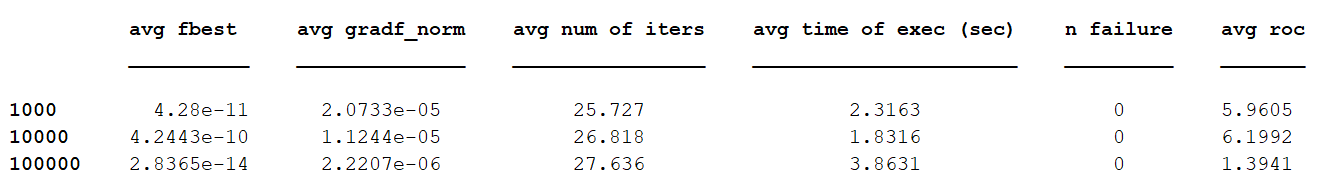
\includegraphics[width = 0.9\textwidth]{img/pb25_MN_table.png}
    \caption{Results obtained by running the Modified Newton method on the problem $25$ using the exact derivatives.}
\end{figure*}

As expected from the theoretical background we have about thhese methods, the Modified Newton method with exact derivatives performs significantly better than the Nealder Mead method. The table shows that the method converges to the minimum point for all dimensionalities tested, and the minimum value found is consistently close to zero. 
This is because the Modified Newton method leverages the gradient and Hessian information, allowing it to make more informed steps towards the minimum and thus to converge in fewer iterations.

However, we can notice that the ratio between the average time of execution and the average number of iterations is smaller for the symplex method. This means that each iteration performed by the Modified Newton method is more high-performance but they are also more costly. 

\medskip
\subsection*{Modified Newton Method - Approximated Derivatives}
Approximating the derivatives of the function $F(\mathbf{x})$ using finite differences is more challenging than it appears due to potential numerical cancellation issues, which can occur when subtracting two nearly equal quantities. Additionally, we aim to derive a formula that minimizes computational cost.

As done previously we will first consider the case in which the dimensionality $n$ is an even integer and then we will specify what changes if $n$ is an odd number.

Let's begin by approximating the first order derivatives by using the centered finite difference formula with increment $h_k$. We keep track of the subscript $k$ in order to derive formula which are valid both for the case with costant increments and the case in which the increments depend on the components respect to which we are differentiating.
The general formula is
$$ \frac{\partial F }{\partial x_k} (\mathbf{x}) \approx \frac{F(\mathbf{x} + h_k \vec{e}_k) - F(\mathbf{x} - h_k \vec{e}_k)}{2h_k} = 
\frac{\sum_{i = 1}^{n} f_i(\mathbf{x} + h_k \vec{e}_k)^2 - \sum_{i = 1}^{n} f_i(\mathbf{x} - h_k \vec{e}_k)^2}{4h_k}$$
but it would not be much wise to apply it directly to out problem because it would be unnecessary to evaluate all the terms $f_i^2(\mathbf{x})$ which are not affected by the varation of the $k$-th component of the vector $\mathbf{x}$.
In particular, we can notice that if we are differentiating with respect to an even component the only term we need to compute is $f_{k-1}^2()$, while if we are differentiating with respect to an odd component we only need to expand the terms $f_k^2()$ and $f_{k+1}^2()$.
Omitting the calculus, we obtain the following formula
\begin{align*}
    \frac{\partial F}{\partial x_k} (\mathbf{x}) &\approx \frac{f_{k-1}^2(\mathbf{x} + h_k \vec{e}_k) - f_{k-1}^2(\mathbf{x} - h_k \vec{e}_k)}{4h_k} = \frac{- 40h_k (10x_{k-1}^2 - 10x_k)}{4h_k} \quad  &\mod(k,2)  = 0 \\
    \frac{\partial F}{\partial x_k} (\mathbf{x}) &\approx \frac{f_{k}^2(\mathbf{x} + h_k \vec{e}_k) - f_{k}^2(\mathbf{x} - h_k \vec{e}_k) + f_{k+1}^2(\mathbf{x} + h_k \vec{e}_k) - f_{k+1}^2(\mathbf{x} - h_k \vec{e}_k)}{4h_k} \\ &= \frac{80x_k h_k (10x_k^2 + 10 h_k^2 -10x_{k+1}) - 4h_k (x_k -1)}{4h_k} \quad &\mod(k,2) = 1
\end{align*}

If $n$ is an odd number, the approximation of $\frac{\partial F}{\partial x_1} (\mathbf{x})$ will slightly change into 
\begin{align*}
\frac{\partial F}{\partial x_1} (\mathbf{x}) & \approx  \frac{f_{1}^2(\mathbf{x} + h_1 \vec{e}_1) - f_{1}^2(\mathbf{x} - h_1 \vec{e}_1) + f_{2}^2(\mathbf{x} + h_1 \vec{e}_1) - f_{2}^2(\mathbf{x} - h_1 \vec{e}_1) + f_n^2(\mathbf{x} + h_1 \vec{e}_1) - f_n^2(\mathbf{x} - h_1\vec{e}_1)}{4h_1} \\ &
 = \frac{80x_1 h_1(10x_1^2 + 10 h_1^2 -10x_{2}) - 4h_1 (x_1 -1) -40h_1 (10x_n^2 - 10x_1) }{4h_1}
\end{align*}

For what concerns the second order derivatives, we can apply a similar reasoning based on negletting the terms $f_i^2(\mathbf{x})$ which are not affected by the variation of the $k$-th component of $\mathbf{x}$ but starting from the general formula
$$ \frac{\partial^2 F}{\partial x_i \partial x_j} (\mathbf{x})  = \frac{F(\mathbf{x} + h_i \vec{e}_i + h_j \vec{e}_j) - F(\mathbf{x} + h_i \vec{e}_i) - F(\mathbf{x} - h_j \vec{e}_j) + F(\mathbf{x})}{h_i h_j}$$
Due to the particular structure of the problem we are considering, many second order derivatives are zero, thus we are going to approximate solely the ones we know are not null.
\begin{align*}
    & \frac{\partial^2 F}{\partial x_k^2} (\mathbf{x}) \approx \frac{f_{k-1}^2 (\mathbf{x} + 2h_k \vec{e}_k) - 2 f_{k-1}^2 (\mathbf{x} + h_k \vec{e}_k) + f_{k-1}(\mathbf{x})}{2h_k^2} = \frac{200h_k^2}{2 h_k^2}, & \mod(k,2) = 0 \\
    & \frac{\partial^2 F}{\partial x_k^2} (\mathbf{x}) \approx \frac{f_{k}^2 (\mathbf{x} + 2h_k \vec{e}_k) - 2 f_{k}^2 (\mathbf{x} + h_k \vec{e}_k) + f_{k}(\mathbf{x}) + f_{k+1}^2 (\mathbf{x} + 2h_k \vec{e}_k) - 2 f_{k+1}^2 (\mathbf{x} + h_k \vec{e}_k) + f_{k+1}(\mathbf{x})}{2h_k^2} \\
    & \qquad = \frac{40h_k^2 (10x_k^2 - 10x_{k+1}) + 1400 h_k^4 + 2400h_k^3 x_k + 800 x_k h_k^2 + 2h_k^2}{2 h_k^2}, & \mod(k,2) = 1 \\
    & \frac{\partial^2 F}{\partial x_k \partial x_{k+1}} (\mathbf{x}) \approx \frac{f_{k}^2 (\mathbf{x} + h_k \vec{e}_k + h_{k+1} \vec{e}_{k+1}) - f_{k}^2 (\mathbf{x} + h_k \vec{e}_k) - f_{k}^2 (\mathbf{x} + h_{k+1} \vec{e}_{k+1}) + f_{k}(\mathbf{x})}{2h_k h_{k+1}} \\
    & \qquad = \frac{20h_{k+1} (-10h_k^2 - 20h_k x_k)}{2h_k h_{k+1}}, & \mod(k,2) = 1
\end{align*}
We explicitely approximated just the superior diagonal, the inferior one is obtained by imposing the simmetry of the hessian matrix.

If the dimensionality $n$ is an odd number, the changes only concern the term  $\frac{\partial^2 F}{\partial x_1^2} (\mathbf{x})$ and the extremal diagonal which are not null anymore. In particular, these terms become
\begin{align*}
    \frac{\partial^2 F}{\partial x_1^2} (\mathbf{x}) & \approx\frac{40h_1^2 (10x_1^2 - 10x_{2}) + 1400 h_1^4 + 2400h_1^3 x_1 + 800 x_1 h_1^2 + 202h_1^2 }{2 h_k1^2} \\
    \frac{\partial^2 F}{ \partial x_n \partial x_1} & = \frac{\partial^2 F}{ \partial x_1 \partial x_n} \approx \frac{20h_1(-20x_n h_n - 10h_n^2 )}{2h_1 h_n}
\end{align*}


According to what we expect, seeking for the minimum using the approximations of the derivatives affects the performance of the Modified Newton method, expecially for larger values of the increment $h$. From a theoretical point of view, this can be justified because the approximated derivatives are nearer to their analitical value when the increment $h$ is tending toward $0$.
Then, we are not surprised that for $h = 10^{-2}$ the algorithm often converges to a point which value is not very close to $0$ and it needs much more iterations to satisfy the stopping criterion.

\begin{figure}[htbp]
    \centering
    % Prima immagine
    \begin{subfigure}[t]{0.45\textwidth}  % Larghezza del 45% del testo
        \centering
        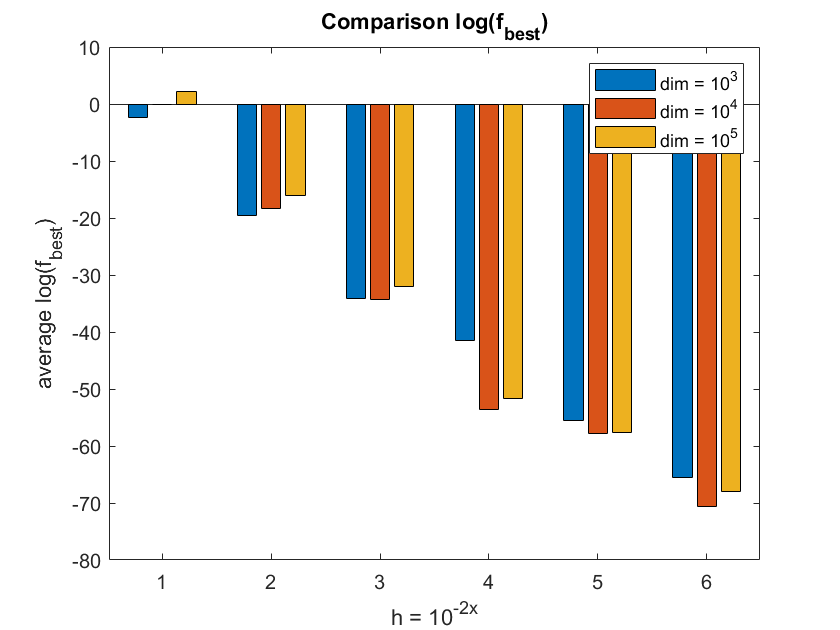
\includegraphics[width=\textwidth]{img/pb25_MN_difffinite_COST_log(fbest).png}
        \caption{Costant Increment $h$}
    \end{subfigure}
    \hspace{1cm} %spaziatura tra le immagini
    % Seconda immagine
    \begin{subfigure}[t]{0.45\textwidth}
        \centering
        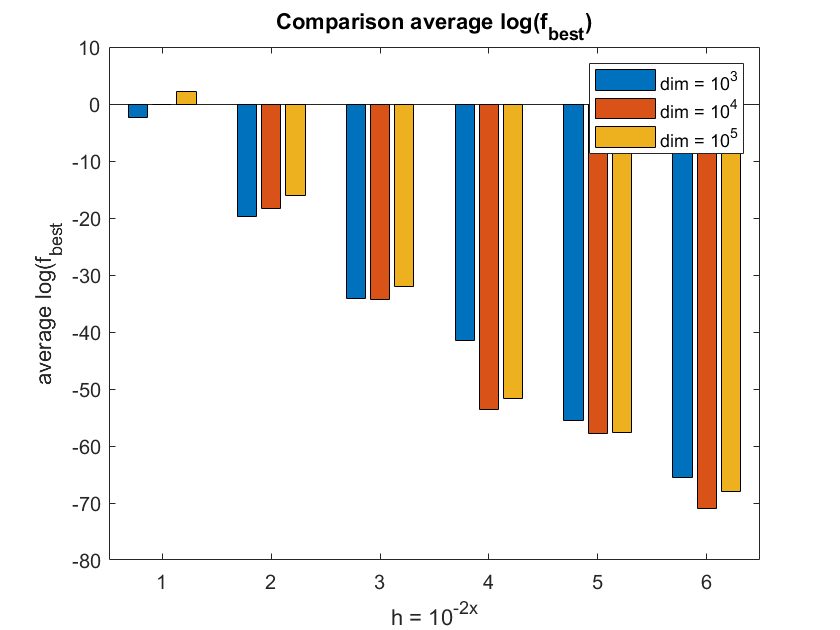
\includegraphics[width=\textwidth]{img/pb25_MN_difffinite_REL_log(fbest).png}
        \caption{Specific Increment }
    \end{subfigure}
    % Didascalia generale
    \caption{ \small Values of the average $\log(f_{best})$ in function of the increment while running the Modified Newton Method with approximated derivatives on the problem $25$.}
    \label{logfbest_difffinite25}
\end{figure}


\begin{figure*}[htbp]
    \centering
    % Prima immagine
    \begin{subfigure}[t]{0.45\textwidth}  % Larghezza del 45% del testo
        \centering
        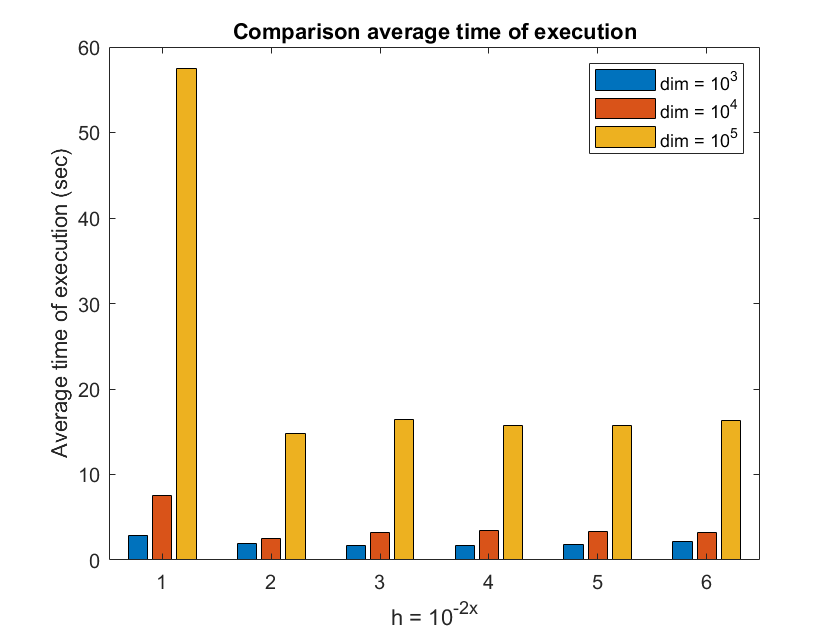
\includegraphics[width=\textwidth]{img/pb25_MN_difffinite_COST_timeofexec.png}
        \caption{Costant Increment $h$}
    \end{subfigure}
    \hspace{1cm} %spaziatura tra le immagini
    % Seconda immagine
    \begin{subfigure}[t]{0.45\textwidth}
        \centering
        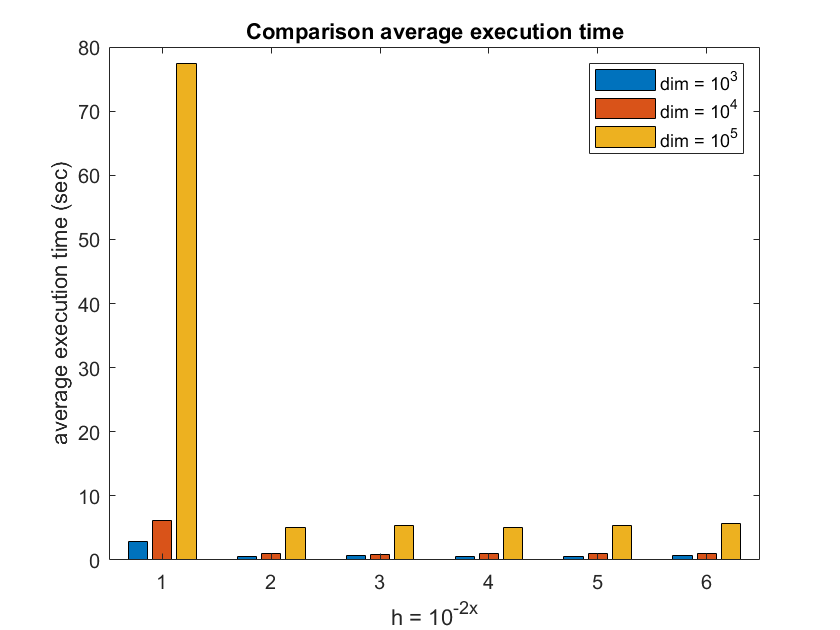
\includegraphics[width=\textwidth]{img/pb25_MN_difffinite_REL_timeofexec.png}
        \caption{Specific Increment }
    \end{subfigure}
    % Didascalia generale
    \caption{ \small Average time of execution in function of the increment $h$  while running the Modified Newton Method with approximated derivatives on the problem $25$.}
\end{figure*}

\begin{figure*}[htbp]
    \centering
    % Prima immagine
    \begin{subfigure}[t]{0.45\textwidth}  % Larghezza del 45% del testo
        \centering
        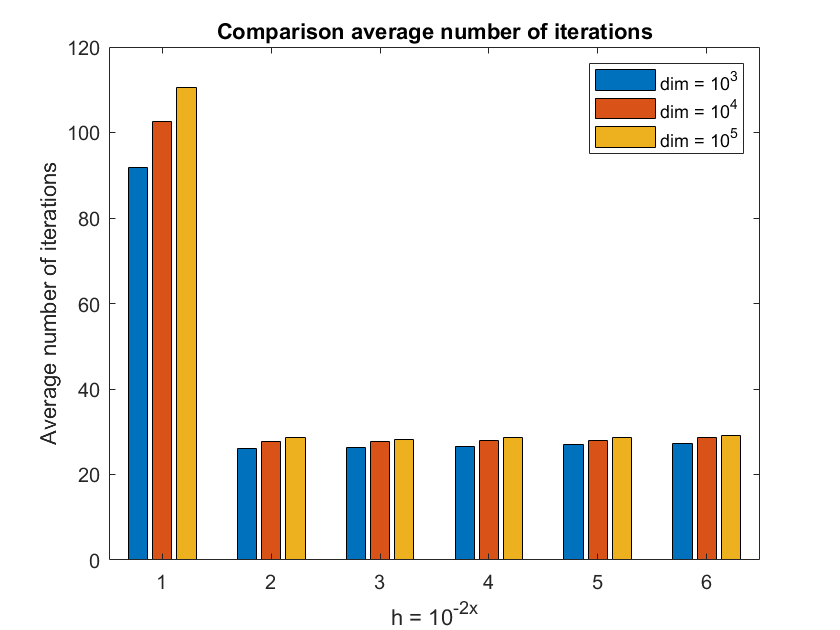
\includegraphics[width=\textwidth]{img/pb25_MN_difffinite_COST_avgiterations.png}
        \caption{Costant Increment $h$}
    \end{subfigure}
    \hspace{1cm} %spaziatura tra le immagini
    % Seconda immagine
    \begin{subfigure}[t]{0.45\textwidth}
        \centering
        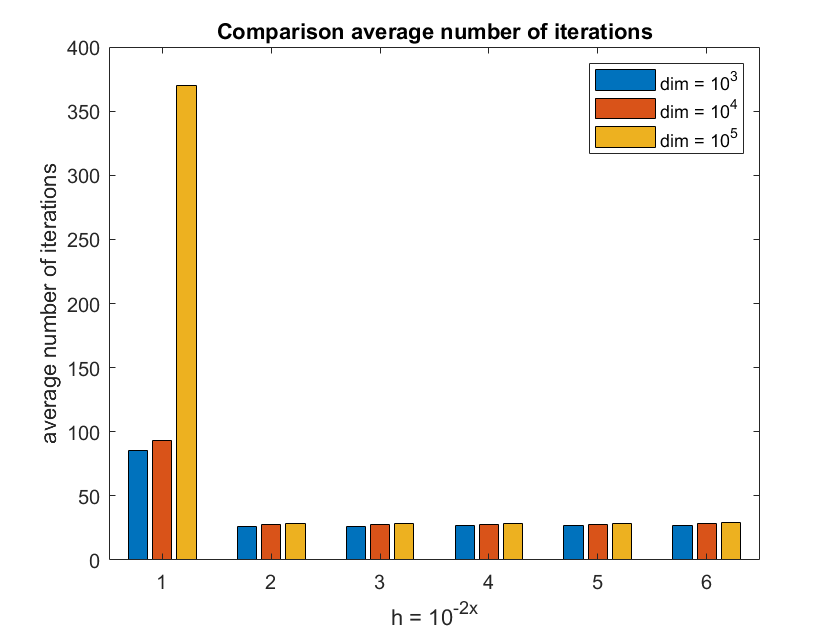
\includegraphics[width=\textwidth]{img/pb25_MN_difffinite_REL_avgiterations.png}
        \caption{Specific Increment}
    \end{subfigure}
    % Didascalia generale
    \caption{ \small Average number of iterations in function of the increment $h$  while running the Modified Newton Method with approximated derivatives on the problem $25$.}
\end{figure*}


\begin{figure*}[htbp]
    \centering
    % Prima immagine
    \begin{subfigure}[t]{0.45\textwidth}  % Larghezza del 45% del testo
        \centering
        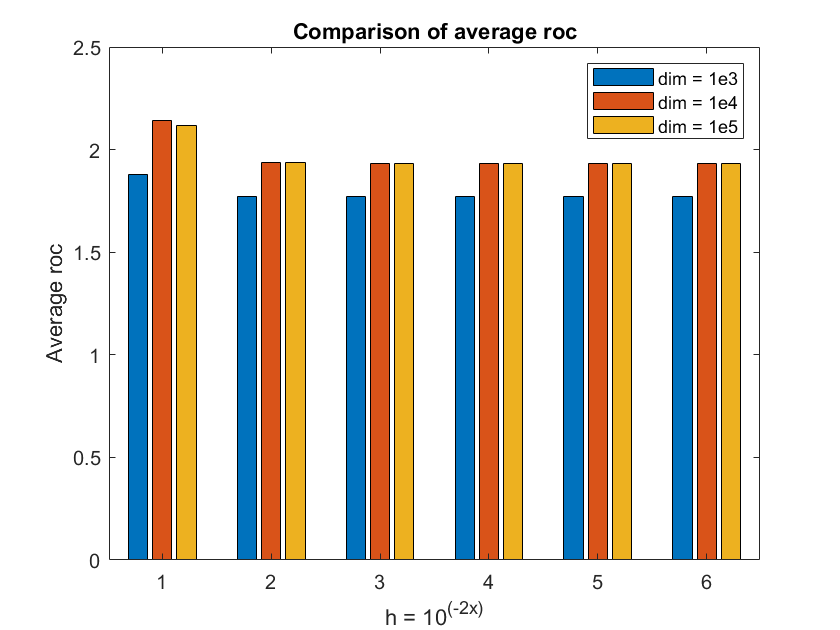
\includegraphics[width=\textwidth]{img/pb76_MN_difffinite_COST_rateofconv.png}
        \caption{Costant Increment $h$}
    \end{subfigure}
    \hspace{1cm} %spaziatura tra le immagini
    % Seconda immagine
    \begin{subfigure}[t]{0.45\textwidth}
        \centering
        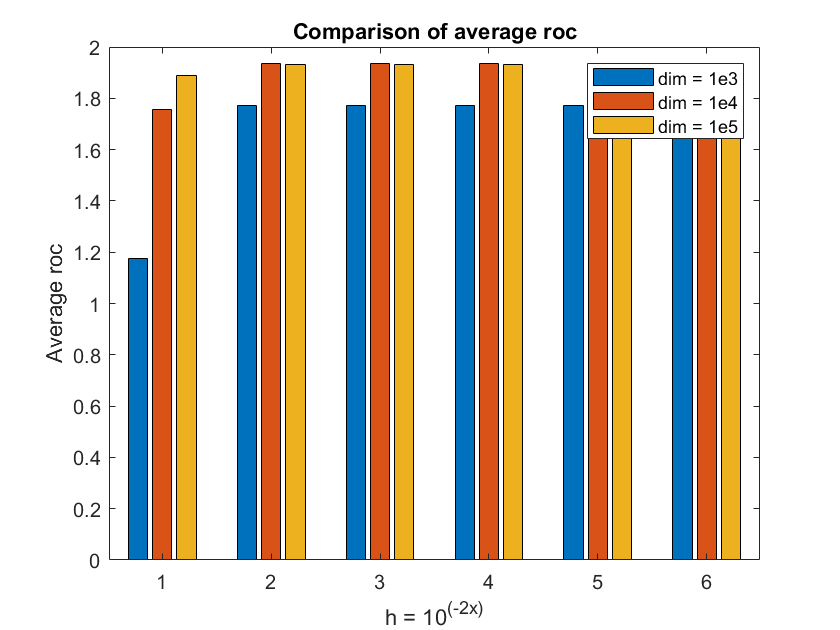
\includegraphics[width=\textwidth]{img/pb76_MN_difffinite_REL_rateofconv.png}
        \caption{Specific Increment }
    \end{subfigure}
    % Didascalia generale
    \caption{ \small Average values of the experimental rate of convergence in function of the increment $h$  while running the Modified Newton Method with approximated derivatives on the problem $25$.}
\end{figure*}


